\chapter{Descripción del entorno de trabajo}
\section{Resumen}

En este capítulo se explica la metodología de trabajo, el desarrollo de los bloques que componen el diagrama general y se realiza una breve introducción al software empleado para utilizar la arquitectura del generador de chirp, como así también a las pruebas de funcionamiento y verificación del mismo.

\subsection{Método de diseño}

El desarrollo se basa en el siguiente flujo:

\begin{enumerate}
    \item \textbf{Cálculos iniciales:} Se inicia con los cálculos de los bloques. Una vez obtenido el valor teórico se continúa con el diseño del bloque calculado, considerando las especificaciones iniciales.
    
    \item \textbf{Simulación del funcionamiento de los bloques:} Tras calcular los bloques se procede a la simulación de cada uno de los módulos por separado; estas simulaciones resultan de gran importancia para corroborar el cálculo teórico inicial.
    
    \item \textbf{Optimización de las simulaciones obtenidas:} Si el modelo teórico difiere de la simulación realizada, se utilizan las herramientas adecuadas para cumplir con las especificaciones iniciales.

    \item \textbf{Construcción de los bloques necesarios:} Una vez comparado el resultado teórico con lo simulado y optimizado, se procede al desarrollo de las partes del generador de chirp.

    \item \textbf{Medición y verificación de los bloques construidos:} Tras medir cada circuito por separado, se contrasta el resultado obtenido con los resultados teóricos y simulados para asegurar el funcionamiento completo del sistema.
       
    \item \textbf{Pruebas finales:} Validan el comportamiento global en distintos escenarios operativos, analizando:
    \begin{itemize}
        \item \textbf{Linealidad del chirp} (clave para no perder resolución en rango).
        \item \textbf{Robustez y ruido de fase}.
        \item \textbf{Límites de la arquitectura} (máxima tasa de barrido $S = \frac{B}{T_c}$).
        \item \textbf{Desempeño general.}
    \end{itemize}
\end{enumerate}

\subsection{Presentación del proyecto completo}
El proyecto está formado por el generador de chirp, compuesto por la placa de evaluación del sintetizador ADF4159EB3Z, el filtro de lazo, el VCO y el divisor de potencia. Por otra parte se encuentra el filtro Hairpin, que tiene la función de filtrar la señal transmitida eliminando las componentes de menor y mayor orden generadas.

\begin{figure}[H]
    \centering
    
\includegraphics[width=0.8\linewidth]{imagenes/diagrama_sistema_completo.png}
    \caption{Sistema completo del proyecto a desarrollar. (Fuente: Propia).}
    \label{fig:diagrama_sistema_completo}
\end{figure}

\subsection{Generador de Chirp FMCW}

El generador de \textit{chirp} es el encargado de sintetizar la señal modulada en frecuencia de forma lineal (\textit{LFM - Linear Frequency Modulation}) que utiliza el radar FMCW. La arquitectura se divide en bloques funcionales que garantizan una generación precisa, lineal y sincronizada de la rampa de frecuencia.

El sistema propuesto para la generación de la señal \textit{chirp} se fundamenta en una arquitectura de sintetizador de frecuencia basada en un Lazo de Enganche de Fase (PLL). A diferencia de los sintetizadores convencionales de frecuencia fija, este diseño emplea un PLL configurado para lograr la modulación lineal en frecuencia, permitiendo el control preciso de la frecuencia de salida en función del tiempo.

La generación de la rampa se ejecuta mediante la modulación del divisor de frecuencia en el lazo de realimentación, lo que obliga al oscilador controlado por tensión (VCO) a seguir una trayectoria de frecuencia lineal predefinida. Este método garantiza la coherencia de fase y la repetibilidad del \textit{chirp}, parámetros críticos para asegurar una resolución espacial constante y una baja degradación del espectro en el proceso de recepción.

La arquitectura implementada permite alcanzar un ancho de banda de barrido de 300~MHz con un período de repetición de 1~ms, balanceando la complejidad del diseño de lazo de control con los requisitos de linealidad exigidos por la aplicación radar. En este proyecto se usará la placa de evaluación del ADF4159 para desarrollar el PLL con posibilidad de modulación con aplicación en radares FMCW.

\begin{figure}[H]
    \centering
    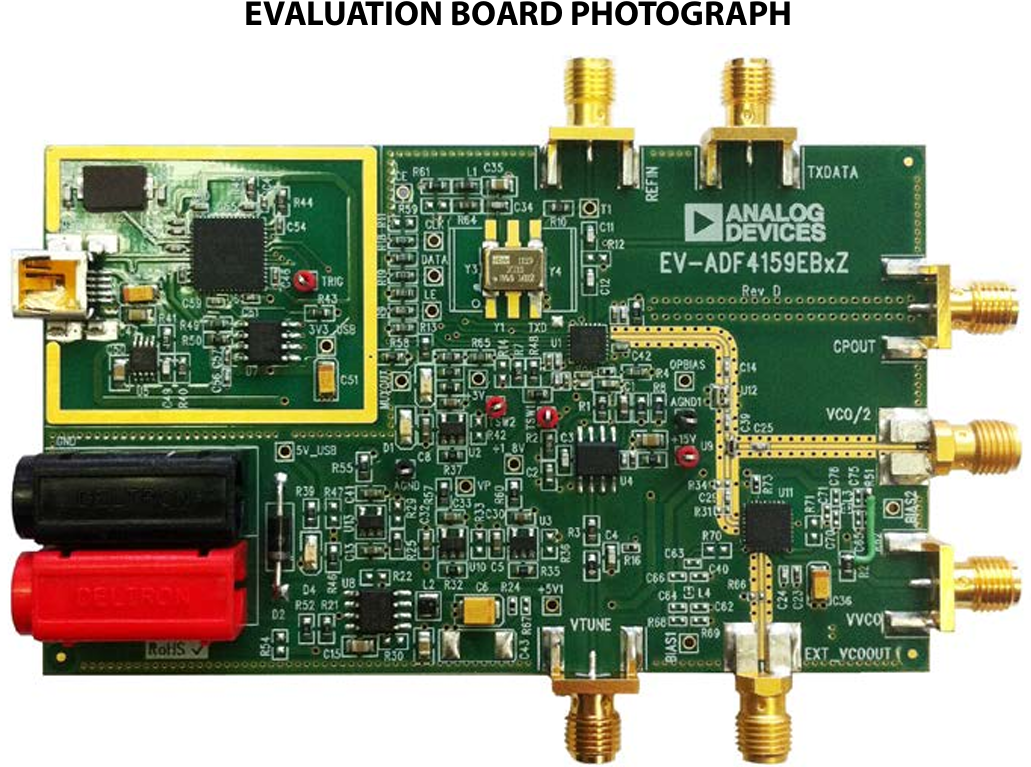
\includegraphics[width=0.8\linewidth]{imagenes/EV-ADF4159EB3Z.png}
    \caption{Placa de evaluación EV-ADF4159EB3Z del sintetizador ADF4159. (Fuente: \cite{ADF4159EB3Z}).}
    \label{fig:ev_adf4159}
\end{figure}

\subsection{Herramientas de Diseño y Simulación}
El diseño y la optimización de la arquitectura propuesta han sido respaldados por el uso de herramientas de software especializadas, garantizando la precisión técnica antes de la fabricación del prototipo.

Para el modelado del comportamiento dinámico del sintetizador y el diseño del filtro de lazo activo, se empleó la herramienta \textit{ADIsimPLL} de Analog Devices. Este software permitió simular la respuesta del lazo cerrado, incluyendo la evaluación del ruido de fase y el tiempo de establecimiento de la rampa, asegurando que los componentes del filtro cumplieran con los requisitos de ancho de banda y estabilidad.

Por otro lado, para la síntesis y caracterización de los circuitos de radiofrecuencia complementarios —tales como el filtro \textit{hairpin}, el divisor de potencia y el VCO—, se utilizó el software \textit{Advanced Design System} (ADS) de Keysight Technologies. Mediante simulaciones electromagnéticas y de parámetros S, esta plataforma permitió optimizar la adaptación de impedancias en las líneas de transmisión y verificar la respuesta en frecuencia de los filtros.

Adicionalmente, la configuración y programación del sintetizador PLL ADF4159 se realizó mediante el software de control proporcionado por Analog Devices. Esta herramienta fue fundamental para determinar los parámetros de división fraccional, gestionar los registros de control interno y definir las temporizaciones precisas necesarias para conformar el perfil de barrido de frecuencia (\textit{chirp}) lineal de 300~MHz en 1~ms, permitiendo validar la comunicación serial y la lógica de programación antes de su implementación en el hardware definitivo.

\section{Especificaciones técnicas del generador de chirp}

La señal de salida debe presentar un barrido lineal de frecuencia dentro de la banda de operación definida para el sistema. En particular, se estableció una frecuencia central de aproximadamente $1{,}7~\mathrm{GHz}$ y un ancho de banda de barrido de $300~\mathrm{MHz}$. De esta manera, la señal debe recorrer el intervalo comprendido entre $1{,}55~\mathrm{GHz}$ y $1{,}85~\mathrm{GHz}$.

En la Tabla~\ref{tab:especificaciones_chirp} se resumen las principales especificaciones técnicas consideradas para el diseño.

\begin{table}[h]
\centering
\begin{tabular}{lc}
\hline
\textbf{Parámetro} & \textbf{Especificación} \\
\hline
Frecuencia central & $1{,}7~\mathrm{GHz}$ \\
Ancho de banda de barrido & $300~\mathrm{MHz}$ \\
Frecuencia inicial & $1{,}55~\mathrm{GHz}$ \\
Frecuencia final & $1{,}85~\mathrm{GHz}$ \\
Tiempo de chirp & $1~\mathrm{ms}$ \\
Pendiente de frecuencia & $3\times10^{11}~\mathrm{Hz/s}$ \\
Frecuencia de referencia del PFD & $50~\mathrm{MHz}$ \\
Ancho de banda del PLL & $\approx 290~\mathrm{kHz}$ \\
Tipo de modulación & Barrido lineal de frecuencia \\
Arquitectura & PLL + VCO \\
\hline
\end{tabular}
\caption{Especificaciones técnicas del generador de chirp.}
\label{tab:especificaciones_chirp}
\end{table}

Estas especificaciones definen los principales requerimientos de diseño que deben cumplirse durante las etapas posteriores de simulación, implementación y caracterización experimental del generador.

\section{Especificaciones técnicas del filtro Hairpin}

El filtro pasabanda debe permitir el paso de la señal de barrido generada por el sintetizador, suprimiendo las componentes armónicas y las señales espurias fuera de la banda de interés. En concordancia con el generador de chirp, se estableció una frecuencia central de $1{,}7~\mathrm{GHz}$ y un ancho de banda fraccional que garantice una transmisión plana en el intervalo de $1{,}55~\mathrm{GHz}$ a $1{,}85~\mathrm{GHz}$, manteniendo una adecuada selectividad y adaptación de impedancia en los puertos.

En la Tabla~\ref{tab:especificaciones_hairpin} se resumen las principales especificaciones técnicas consideradas para el diseño del filtro.

\begin{table}[H]
\centering
\begin{tabular}{lc}
\hline
\textbf{Parámetro} & \textbf{Especificación} \\
\hline
Frecuencia central ($f_0$) & $1{,}7~\mathrm{GHz}$ \\
Banda de paso ($BW$) & $380~\mathrm{MHz}$ \\
Frecuencia de corte inferior ($f_1$) & $1{,}510~\mathrm{GHz}$ \\
Frecuencia de corte superior ($f_2$) & $1{,}890~\mathrm{GHz}$ \\
Tipo de respuesta & Chebyshev \\
Orden del filtro ($n$) & $5$ \\
Rizado en la banda de paso ($A$) & $0{,}5~\mathrm{dB}$ \\
Impedancia de referencia ($Z_0$) & $50~\Omega$ \\
Topología & Microstrip (líneas acopladas en horquilla) \\
\hline
\end{tabular}
\caption{Especificaciones técnicas del filtro pasabanda Hairpin.}
\label{tab:especificaciones_hairpin}
\end{table}

Estas especificaciones definen los principales requerimientos de diseño que deben cumplirse durante las etapas posteriores de cálculo analítico, simulación electromagnética y fabricación del filtro.